\interlude{The Rosenpass Protocol}
\section{The Rosenpass Protocol}

\begin{frame}{The Rosenpass Protocol}
  \begin{columns}[fullwidth,c]
    \begin{column}{.5\linewidth}
\includegraphics[width=\linewidth]{scientific/rosenpass-whitepaper-key-exchange-protocol.pdf}
    \end{column}

    \begin{column}{.48\linewidth}
      \begin{itemize}
        \item Authenticated key exchange
        \item Post-quantum Noise-IK
        \item Three KEM operations
        \item No use of signatures
        \item Improvement upon \say{Post-quantum WireGuard} (eprint 2020/379)
      \end{itemize}
    \end{column}
  \end{columns}
\end{frame}

\begin{frame}{Three KEM operations}
  \centering
  \includegraphics[height=.85\textheight,page=6,clip,trim=0 170 0 70]{scientific/rosenpass-wireguard-key-exchanges-nike-kem.pdf}
\end{frame}

\begin{frame}{Three KEM operations…interleaved}
  \begin{columns}[fullwidth,c]
    \begin{column}{.30\linewidth}
      \includegraphics[height=.85\textheight,page=7,clip,trim=95 190 95 70]{scientific/rosenpass-wireguard-key-exchanges-nike-kem.pdf}
    \end{column}
    \begin{column}{.45\linewidth}
      \includegraphics[height=.60\textheight,page=5,clip,trim=95 205 95 90]{scientific/rosenpass-wireguard-key-exchanges-nike-kem.pdf}
    \end{column}
  \end{columns}
\end{frame}

\begin{frame}{in essence, gives you the Rosenpass protocol}
  \centering
  \includegraphics[height=.85\textheight]{scientific/rosenpass-whitepaper-key-exchange-protocol.pdf}
\end{frame}

\begin{frame}{Spot the biscuit}
  \begin{columns}[fullwidth,c]
    \begin{column}{.48\linewidth}
    \centering
    \vspace{.8em}
    \includegraphics[height=.39\linewidth,clip,trim=110 120 0   0]{scientific/rosenpass-whitepaper-message-types.pdf}
    \\ \includegraphics[height=.35\linewidth,clip,trim=350 0 0   150]{scientific/rosenpass-whitepaper-message-types.pdf}
    \end{column}

    \begin{column}{.48\linewidth}
        \centering
        InitHello achieves no initiator authentication at all.
        \\[.8em]
        It is trivial to forge this package, displacing any legitimate ongoing handshake.
        \\[.8em]
        Therefor, the responder state is stored in an encrypted cookie called "biscuit", not in responder memory.
        \\[.8em]
        This does not prevent replay or forgery attacks, but they don't threaten security or abort the protocol.

    \end{column}
  \end{columns}
\end{frame}

\begin{frame}{Hybridization through combination with WireGuard}
  \begin{columns}[fullwidth,c]
    \begin{column}{.22\linewidth}
      \flushright
      Rosenpass
    \end{column}
    \begin{column}{.65\linewidth}
      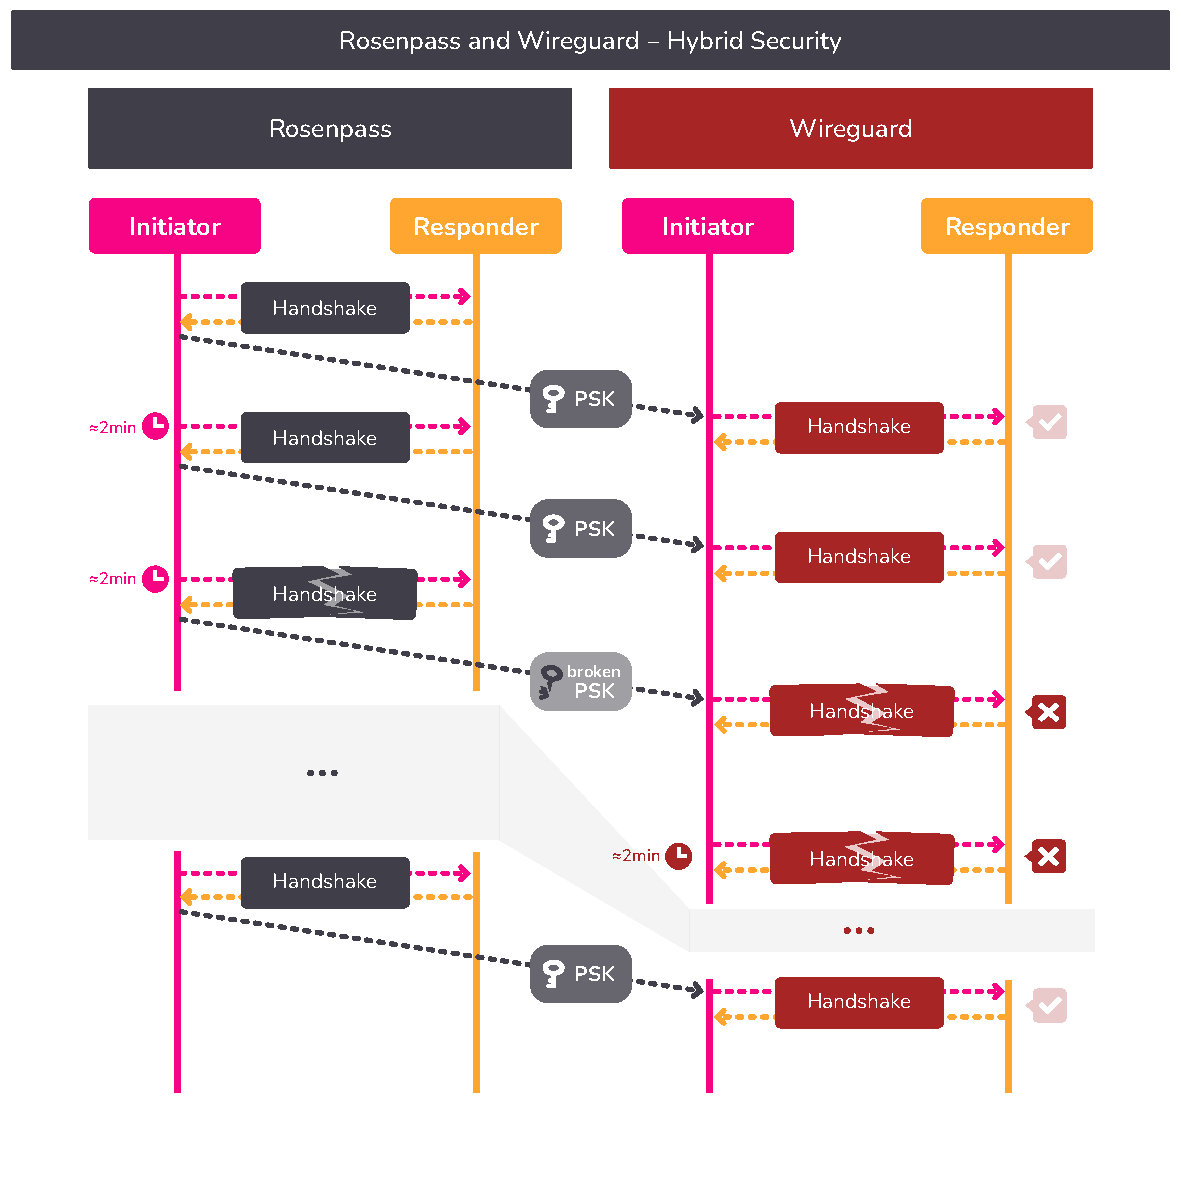
\includegraphics[height=.85\textheight,clip,trim=0 50 0 93 ]{scientific/rosenpass-wireguard-hybrid-security.pdf}
    \end{column}
    \begin{column}{.25\linewidth}
      \flushleft
      WireGuard
    \end{column}
  \end{columns}
\end{frame}

\begin{frame}{}
  \centering
  \only<1>{
    \includegraphics[height=.892\textheight]{scientific/rosenpass-whitepaper-message-types.pdf}
  }
  \only<2>{
    \includegraphics[height=.95\textheight]{scientific/rosenpass-whitepaper-hashing-tree.pdf}
  }
  \only<3>{
    \includegraphics[height=.95\textheight]{scientific/rosenpass-whitepaper-message-handling-code.pdf}
  }

  \raggedright
  \footnotesize
  \hspace{-2.5em} rosenpass.eu/whitepaper.pdf
\end{frame}

\begin{frame}{Security modeling}
  \begin{columns}[c]
    \begin{column}{.5\linewidth}
     \rlap{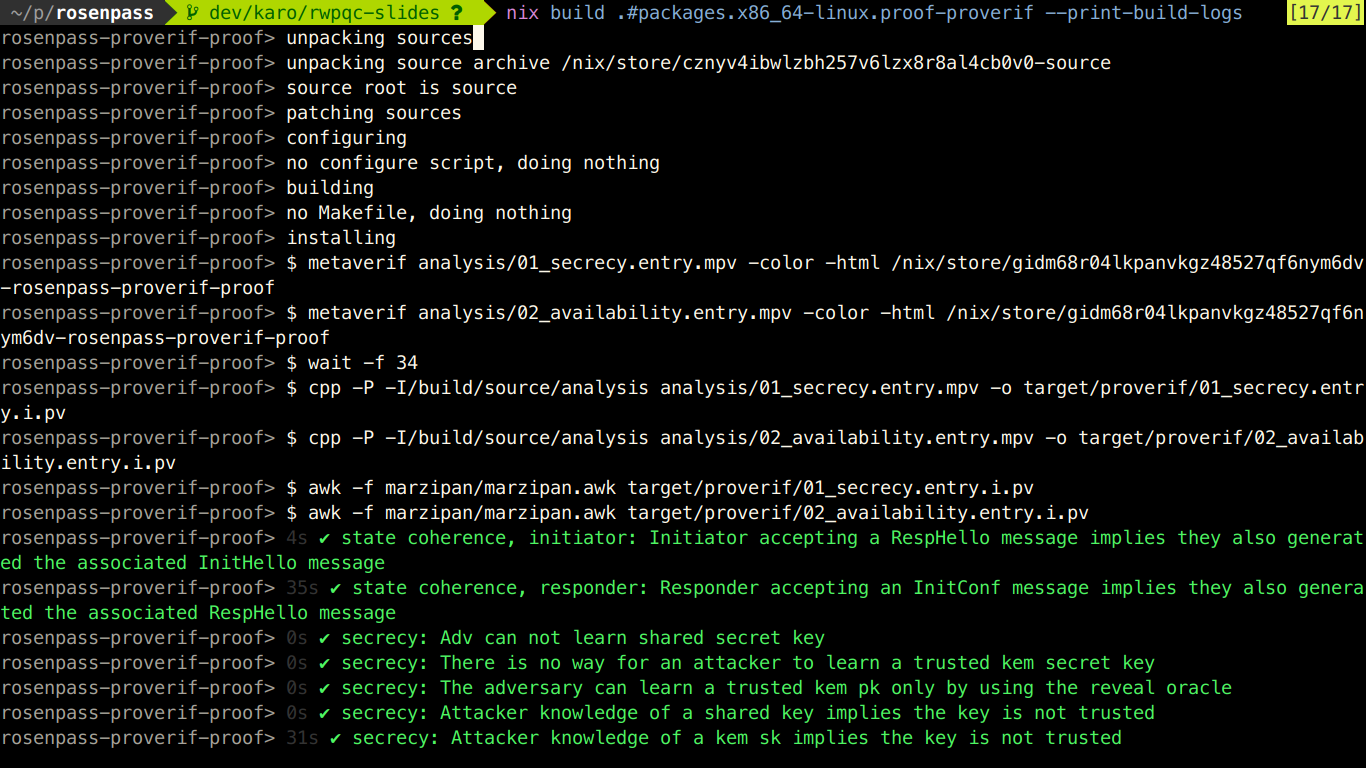
\includegraphics[keepaspectratio,height=.85\textheight]{graphics/2023-03-20-symbolic-analysis-screenshot.png}}
    \end{column}
	\pause
    \begin{column}{.5\linewidth}
    \tikz\node[rectangle,fill opacity=1,fill=white,minimum height=.85\textheight, text width=\linewidth]{
      \begin{itemize}
        \item Mechanized verification using ProVerif
        \item Proofs treated as part of the codebase
        \item Mechanized proof in the computational model is something we want
      \end{itemize}};
    \end{column}
  \end{columns}
\end{frame}
